\documentclass{llncs}
\usepackage{times}
\usepackage[utf8]{inputenc}
\usepackage[T1]{fontenc}
\usepackage[portuguese]{babel}

% Comentar para not MAC Users
%\usepackage[applemac]{inputenc}

\usepackage{a4}
%\usepackage[margin=3cm,nohead]{geometry}
\usepackage{epstopdf}
\usepackage{graphicx}
\usepackage{fancyvrb}
\usepackage{amsmath}
\usepackage{subfig}
%\renewcommand{\baselinestretch}{1.5}

\graphicspath{ {./} }

\begin{document}
\mainmatter

\date{4 Outubro}
\title{IoT - Segurança e Desafios}

\titlerunning{}

\author{Filipe Monteiro \and Bruno Martins \and Márcio Sousa}

\authorrunning{Autor1 \and Autor2 \and Autor3}

\institute{
University of Minho, Department of  Informatics, 4710-057 Braga, Portugal\\
e-mail: \{a80229,a80410,a82400\}@alunos.uminho.pt
}


\bibliographystyle{splncs}

\maketitle
\begin{abstract}
O interesse crescente em dispositivos inteligentes para casas/cidades, em que tudo esteja ligado em rede para de alguma maneira facilitar a nossa vida tem criado alguns problemas. Com a arquitura atual da internet, as comunicações protocolares baseadas no IP vão permitir a conectividade entre dispositivos no contexto de IoT. Desta forma surgem vários desafios e problemas no que toca à segurança das redes. Para  melhorar o aspeto de segurança propomos uma arquitetura SD-VPN como uma solução possível em que os aparelhos são alocados numa camada da VPN. Quanto aos desafios neste momento os mais preocupantes são a privacidade das redes, o anonimato e a falta de tempo de vida em que um dispositivo se mantém atualizado.
\end{abstract}

\section{Introdução}

%N�o esquecer de referenciar apropriadamente...
A IoT  (Internet of Things) é uma infraestrutura de rede dinâmica
e global com capacidades de autoconfiguração, baseada em protocolos de comunicação. Na IoT, os objetos devem se
tornar participantes ativos em processos de negócio, sociais, onde deverão ser capazes de comunicar entre si, trocar informações recolhidas do que os rodeia, reagindo automaticamente aos eventos do mundo real, bem como influencia-lo sem intervenção direta do ser humano.
No entanto, segurança e privacidade deverão sempre ser consideradas. Neste contexto insere-se o presente ensaio: a comunicação necessária entre as coisas ou objetos, efetivamente realizadas atraves das interfaces de rede, abre possibilidades de ataques externos ou internos de segurança. Os atacantes buscam entao explorar vulnerabilidades para poderem influenciar o comportamento ou obter o controle do sistema. 


\section{Vulnerabilidades}
IoT distingue-se das redes de computadores tradicionais em vários aspetos. Por exemplo, a sua escala é maior, sendo composta por centenas ou milhares de nós.
Idealmente, os nós da IoT são compostos por Sistemas Embutidos (SE's) de baixo custo, a fim de reduzir o valor final de produtos. Ora, os SE's possuem poucos recursos computacionais (processamento,
memoria, entre outros) e não são capazes de executar sistemas “pesados”. Assim sendo, para 
ajudar nessa questão, os sistemas para IoT são frequentemente desenvolvidos em linguagens de programação eficientes, tal como C.
Contudo, sistemas desenvolvidos nesta linguagem são mais inseguros: torna os mais “leves” (melhores para SE's) mas com um problema: mais vulneráveis. Uma das vulnerabilidades de C está no facto de a linguagem não realizar certas verificações. Uma delas é, por exemplo, o limites dos arranjos, surgindo o perigo de ataque por
Buffer Overflow, um dos ataques mais comuns a sistemas
computacionais. E mecanismos de segurança contra ataques de BOF presentes em PC's, muitas vezes não estão presentes em SE's. Outro fator que afeta a segurança é que tarefas na IoT são normalmente realizadas em conjunto. Assim a natureza desses sistemas é alterada, passando a ser distribuídos. Como os nós colaboram, também trocam mais mensagens, aumentando a possibilidade de potenciais ataques.

A maioria dos ataques externos podem ser evitados com o uso de cifras e
códigos de autenticação de mensagens. Existem, no campo da literatura, diversas propostas capazes de proteger uma rede contra essa classe de ataques – por exemplo, SSL/TLS5 para comunicação fim-a-fim em redes tradicionais. Neste modelo, quando uma mensagem é
recebida, é verificada a sua validade e apenas é tratada pelo sistema se a verificação for bem sucedida.\cite{Fernando} \cite{Jorge}

\section{Segurança SD-VPN em IoT}

%UNCOMMENT se necess�rio
%De acordo com o ilustrado na Figura~\ref{fig:controller}
%% Exemplo para inser��o de uma figura
%\begin{figure}
%\begin{center}
%\includegraphics[scale=0.40]{figura.pdf} 
%\end{center}
%\caption{\label{fig:controller}Architecture of the unified QoS metric fuzzy controller.}
%\end{figure} 

Atualmente a maioria  das redes VPN são construidas manualmente o que faz com que isso não só seja caro como também demorado devido às configurações possíveis. Neste contexto de IoT, é util complementar as redes VPN com SDN, o chamado SD-VPN, fazendo com que em vez de serem criados serviços VPN manualmente, quando um cliente se junta ao sistema, esta (a VPN) seja criada automaticamente.\cite{Linda} \par
SDN é uma arquitetura de rede que consiste em dividir a rede por camadas permitindo que esta seja diretamente programável, facilmente adaptada e de baixo custo. A estrutura basea-se numa camanda aplicacional de alto nível (API), esta comunica com uma camada de controlo da rede, que por sua vez comunica com uma camada de infrastruturas através do sitema OpenFlow. OpenFlow é um protocolo comunicacional que permite à rede determinar o caminho dos pacotes numa rede de switches. Este protocolo também permite switches de vários vendedores, normalmente com diferentes tipos de software e linguagens, que trabalhem em conjunto.\par
O principio básico deste método tem como base a substituição de PE (Provider Edge) routers , utilizados nas redes VPN, por SDN switches que são controlados por SDN controllers utilizando OpenFlow. Desta forma, quando um dispositivo se junta a uma rede VPN é lhe atribuido um conjunto  de metadados únicos que são utilizados para a sua identificação.\par
A metodologia proposta, SD-VPN, usa caracteristicas tanto de SDN com de VPN para melhorar a segurança em dois aspetos: Separação de trafego e Serviço de redes encadeado.\cite{Mirk}\par
Os end-points dos dispositivos IoT estão alocados em vários sítios da VPN na arquitetura SD-VPN. Como segurança básica é utilizado Tunneling, uma tecnologia basica de VPN, semelhante a conecção ponto a ponto que encapsula as comunicações enquanto elas nao chegam ao seu destino. As redes SD-VPN separam o tráfego da rede o que melhora a segurança porque os utilizadores apenas conseguem apenas aceder a uma VPN via \textit{tunnel}. Esta proposta permite separar o trafego mais sensível das outras partes da internet. Como consequência disto, a informação é protegida e previnida a sua fuga. Outra consequência é que utilizadores de uma rede VPN não conseguem transmitir informação a outro utilizador de outra VPN.\par Quanto a Network Service Chaining, não é um conceito totalmente novo, consiste em encadear virtualmente serviços como firewalls, VPNs, uma cadeia pode ser utilizada para tratar dispositivos especificos ou serviços das IoT networks. Desta forma quando é feito um pedido a uma rede é feito um security check ao trafego antes de chegar à VPN, melhorando a segurança geral da rede.\cite{Linda}


\begin{figure}
  \centering
    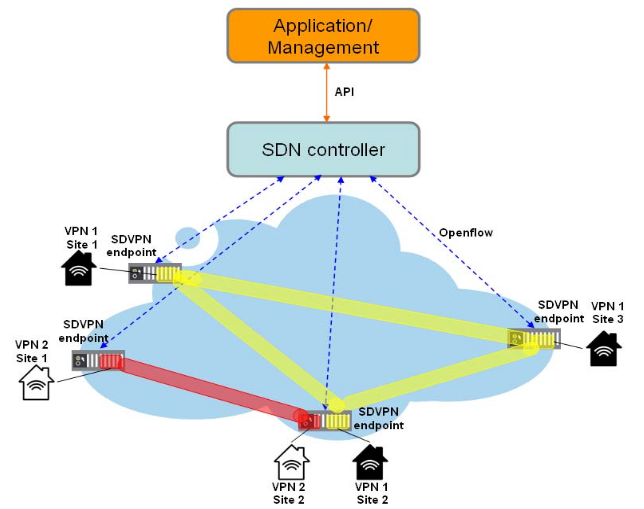
\includegraphics[width=0.4\textwidth]{sdnvpn}
    \caption{Arquitetura SD-VPN \cite{Linda}}
\end{figure}

\section{Desafios existentes na IoT}

No século XXI vivemos constantemente ligados à \textit{rede}: smartphones, computadores, dispositivos da \textbf{IoT} como carros, frigorificos, etc, estão todos interligados entre si. Assim a informação, voluntária ou não, é transmitida e partilhada entre eles, sendo para uso de terceiros ou simplesmente para "controlo" do utilzador.\cite{Fink} Por exemplo, o recente caso do Facebook, onde Mark Zuckerberg estaria a recolher informações dos utilizadores e a vender a terceiros sem o consentimento destes, o que constou uma grande quebra de privacidade.
Aqui serão discutidos alguns dos grandes desafios da IoT para proteção, tanto da rede como do utilizador.

\begin{itemize}
    \item \textbf{Camada Protocolar}

        Apesar de haver um modelo \textit{standard} das camadas protocolares, os fabricantes fazem pequenas alteraçãoes nestas criando a sua própria camada protocolar derivada da principal. Mas isto causa uma série de problemas: para dispositivos comunicarem ambiguamente entre si, tem de haver um consenso. Estudos já realizados por \textit{Ptacek e Newsham} mostram a facilidade de inserção de dados infetados de maneira a atacar apenas determinado dispositivo da rede, apenas por este ter uma arquitetura protocolar ligeiramente modificada. Uma melhoria do Sistema de Deteção de Intrusos (IDS) é obviamente necessária.\par
        Outro ponto fraco atual nestes sistemas protocolares é o \textbf{6LoWPAN} - cria uma camada de adaptação entre o IEEE 802.15.4 e o IPv6, com cabeçalhos específicos que podem ser adicionados ou removidos mediante a sua necessidade, permitindo que seja apenas enviado o que realmente é útil, que devido a diferenças desta implementação em dispositivos da rede podem enviar informação disfarçada, contendo na realidade um \textit{exploit} para este.\newline

    \item \textbf{Identificação na Rede}
        
        A melhor prática para identificar um dispositivo na rede é através de chaves pré-guardadas em memória de apenas leitura, que são usadas para encriptar dados. Mas, esta tem o problema de alto custo de implementação, vulnerabilidade a ataques e constante monotorização destes (consumo continuo de energia - deixa de ser \textit{low power}). Contra esta, existem as PUF (funções físicas não-clonáveis) - gera chaves que diferem de circuito para circuito, dependendo do fabricante, impossível de descobrir através de engenharia reversa - que previnem a falsa autenticação para acesso de dados por outros.
        Mas esta apenas não chega para assegurar a proteção de dados, sendo ainda possível executar ataques para enganar os sistemas de autenticação.\newline
        
        \begin{figure}
            \centering
            \subfloat[Exemplo de uma implementação PUF]{{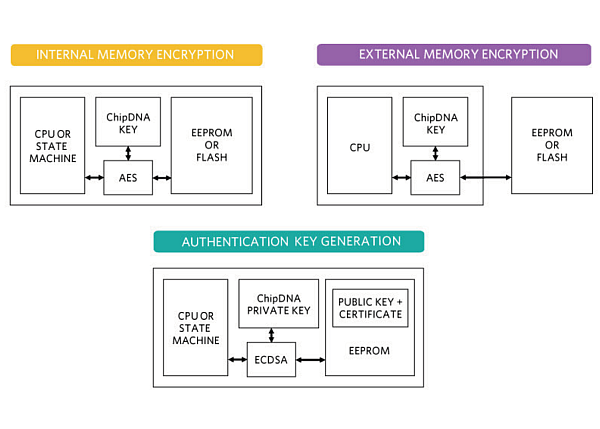
\includegraphics[scale=0.3]{puf}}}
            \qquad
            \qquad
            \qquad
            \subfloat[Uso da Identificação no processo de estabelecer uma ligação segura entre dois dispositivos]{{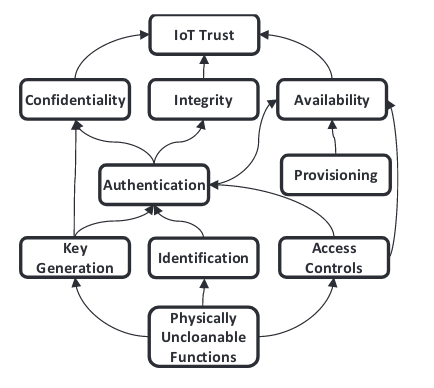
\includegraphics[scale=0.4]{identification_process}}}
            \caption{PUF e Processo de Identificação}
        \end{figure}

    \item \textbf{Tempo de vida dos dispositivos}
        
        No modo geral, um dispositivo possui N anos de suporte e atualizações por parte do fabricante. Mas no fim deste espaço temporal o dispositivo fica para trás em termos de segurança. Muitas redes são enfraquecidas devido a um dispositivo vulnerável nelas, podendo ser atacadas facilmente. Por exemplo, as câmaras CCTV - câmaras usadas em sistemas de vigilância - são dos dispositivos mais vulneráveis numa rede, facilmente acessiveis no mundo real.\par
        Como conseguimos garantir que dados passados entre diversos dispositivos da IoT estejam protegidos da mesma maneira dos dois lados, sendo que cada mantém uma camada de protocolos apenas semelhantes? Ainda mais importante se, um destes estiver \textit{outdated}?
        
    \item \textbf{Privacidade}
        
        Uma possivel solução para garantir a privacidade na rede é melhorar e usar, as chaves SPKI (Infrastrutura simples de chave pública) - uso de chaves que têm associada um certificado de autorização/previlégios - garanta estes 4 aspetos: \cite{Fink}
            \begin{itemize}
                \item \textbf{Anonimato:} o utilizador pode usar recuros sem ser identificado.
                \item \textbf{Pseudoanonimato:} apesar de não ser identificado, tem de ser "responsável" por usá-lo.
                \item \textbf{\textit{Unlinkability}:} o utilizador pode usar vários recursos sem que outros consigam ligar estes ao utilizador.
                \item \textbf{Não Observabilidade:} este pode usar recursos sem que outros observem que estes estejam a ser usados.
            \end{itemize}
        Assim, por exemplo, o uso repetido de um ou vários dispositivos inteligentes não conseguirá gerar identidades que possam ligar ao seu utilizador.\par
        
        Referido no início desta sub-secção, o caso do \textit{Facebook} gerou muita polémica pela quebra de privacidade. Mas no nosso dia-a-dia estamos constantemente a ser monotorizados e a ter perfis traçados, que depois serão usados por terceiros, desde empresas de marketing a serviços governamentais\cite{Fink} (um pouco mais de detalhe mais a baixo).
        Atualmente existem dispositivos inteligentes que, a partir da voz executam ações (por exemplo, \textit{Amazon Echo}. Mas como sabem estes quando responder a um comando de voz por parte do utilizador? Para isto têm de estar constante a gravar o que ouvem e guardar na \textit{cloud}, criando um ou vários perfis do(s) sujeito(s). As empresas de marketing podem então usar os dados para controlo de preços de venda online (um artigo que tenhamos falado muito passa a aparecer com preço mais baixo) e os governos para controlar e vigiar possiveis sujeitos perigosos.
        Segundo este último, a propria \textit{IoT} funciona como um grande sensor dentro da rede onde consegue detetar problemas - aqui vale a pena ter o perfil de todos os individuos no mundo.\par
        Mas apesar dos riscos atenuados com isto, será que vale a pena ter a privacidade e a liberdade controlada por uma entidade externa? Quem deverá ter esta responsabilidade? 

\end{itemize}




%\section{Simulation Scenario}

\section{Conclusão}
Neste trabalho apercebemo-nos do que realmente é a \textit{IoT} e porque é algo tão complexo. Com os vários artigos que analisamos ficamos a entender melhor os grandes problemas que existem nesta, soluções aplicadas no mundo real, SD-VPN para uma melhor segurança de rede e proteção na comunicação de dados entre computadores, combinando várias tecnologias existentes para o encapsulamento da rede, e do quão importante é haver consistência no meio protocolar onde os dipositivos partilham a informação.
Mas ainda existem muitos outros desafios e, com o ritmo de crescimentos atual dos dispositivos na IoT, ficarão cada mais vez mais complexos e possivelmente impossíveis de resolver sem mudanças drásticas no funcionamento desta.\cite{Fink}

%ou inserir directamente os v�rios \bibitem 
\begin{thebibliography}{1}
\bibitem{Linda}
Linda Shi†, Fei Wang‡ and Chung-Horng Lung
\newblock {Improvement of Security and Scalability for IoT
Network Using SD-VPN} (2018)

\bibitem{Mirk}
B. Mirkhanzadeh, N. Taheri, S. Khorsandi,
\newblock {SD-VPN: A SoftwareDefined
Solution for VPN Service Providers} (2016)
\newblock {Boca Raton: Chapman and Hall/CRC Press} (1999)

\bibitem{Fink}
G. Fink, D. Zarzhitsky,T. Carroll, E. Farquhar :
\newblock{Security and privacy grand challenges for the Internet of Things} (2015)

\bibitem{Fernando}
Fernando A. Teixeira, Fernando Pereira, Gustavo Vieira, Pablo Marcondes, Hao Chi Wong, Jose Marcos S. Nogueira, Leonardo B. Oliveira :
\newblock{Siot – Defendendo a Internet das Coisas contra Exploits}

\bibitem{Jorge}
Jorge Granjal, Edmundo Monteiro, Jorge Sá Silva :
\newblock{Security for the Internet of Things: A Survey of Existing Protocols and Open Research Issues}

\end{thebibliography}
\end{document}